\subsection{Methodology}

This section briefly describes the chosen methodology for this project, how the methodology works and how it has been adapted into the project. The prestudy on why Scrum has been chosen, can be found under 'Preliminary Studies'. 

\subsubsection{What is a methodology?}

A project methodology is an approach a project can take to manage all the project activites. There are several types of approaches to take e.g. iterative, incremental, sequential, etc. Regardless of the approach, every project has activites to complete, but they can be scheduled differently.

\subsubsection{What is an agile methodology?}

In a 'normal' project cycle there are activites like analysis, planning, implementation, testing and delivery. How a project schedule these activites depends on the approach. 
The agile approach focuses on helping the team to respond to unpredictability through incremental, iterative work cadences, known as sprints or phases. Agile methodologies are an alternative to waterfall, or traditional sequential development.
Agile development has a known manifesto called 'The Agile Manifesto' that works like this:

\begin{itemize}
	\item Individuals and interactions over processes and tools
    \item Working software over comprehensive documentation
    \item Customer collaboration over contract negotiation
    \item Responding to change over following a plan 
\end{itemize}

The agile manifesto is based on twelve principles that is important to understand before
adapting an agile methodology to a project:

\begin{enumerate}
    \item Customer satisfaction by rapid delivery of useful software
    \item Welcome changing requirements, even late in development
    \item Working software is delivered frequently (weeks rather than months)
    \item Working software is the principal measure of progress
    \item Sustainable development, able to maintain a constant pace
    \item Close, daily cooperation between business people and developers
    \item Face-to-face conversation is the best form of communication (co-location)
    \item Projects are built around motivated individuals, who should be trusted
    \item Continuous attention to technical excellence and good design
    \item Simplicity—the art of maximizing the amount of work not done—is essential
    \item Self-organizing teams
    \item Regular adaptation to changing circumstances
\end{enumerate}

\subsubsection{What is Scrum?}

Scrum is an iterative process with focus on small deliveries and a small set of roles. 
The process defines a self-sustaining team ("The scrum team") that defines the goal for each phase. The goal 
is achieved through small product increments in iteration that normally last for 1-4 weeks. 
All the functions to implement is planned and is added to a listcalled a "Product Backlog". The
functions are normally defined as user stories and are added in a prioritized order. In each increment, 
in Scrum called a "Sprint", there is a sprint meeting where the Scrum team pick user stories from the 
product backlog and add them to a "Sprint Backlog". The sprint backlog is the description of what 
to deliver in the end of the sprint.

In a scrum team there is a small set of roles. There is mainly only three roles: 

\begin{itemize}
    \item {\bf The Product Owner: }The product owner owns the vision and represents the stakeholders
    and shall ensure that the Scrum team are working on the right things from a 
    business perspective. The Product Owner is responsible for the Product Backlog 
    at any time and ensure that the backlog is estimated, prioritized and available to 
    stakeholders and the development team. The backlog list is constantly re-prioritized. 
    \item {\bf The Scrum Master: }The Scrum Master is responsible for the development team and has 
    to ensure that they learn to self-organize, the Product Owner understands his or her role.
    The Scrum Master is responsible for ensuring that they are constantly improving work method 
    and restrospective meetings leading to improvement.
    \item {\bf The Scrum Team: }This team is multidisciplinary and consists typically of 3 to 9 persons.
    It is essential that the team possesses all the skills necessary to create the product increments. 
    Only in this way will they be able to work optimally as a self-organized team. The team takes 
    collective responsibility to create the most value for the stakeholders.
\end{itemize}

A sprint has daily meetings calles a "standup" where all members in the scrum team stand up
to tell what they have done since last standup, what they have finished, what they plan to do this day and
explain any problems they might have. The meeting is very short, its purpose is to give the team a status
update.

After a sprint delivery it is normal to have a "Sprint review" and a "Sprint Retrospective".
For the sprint review the team make a presentation/demonstraion to a group of stakeholders (usually involving the
customer). The purpose of this is to get feedback on the sprint delivery. Because the development
is done in increments, it is possible for the stakeholders to add and change the requirements as well as the implementation done so far. A sprint review then works like a small "aceptance test", because the customer gets the opportunity to say "keep doing what you are doing" or "we want to change what you have done". In this way the stakeholders are always aware of the status and it is an important
way to ensure that the stakeholders will be happy with the final prduct that is developed. 
In other methodologies, the stakeholders are not as involved in the development process, because there is not a 
continous delivery, but a big delivery in the end (as in the waterfall process).

The sprint retrospective is a meeting after the sprint review where the team members talk about what 
the team should start doing, stop doing and continue doing. The purpose of this meeting is to always 
get the members to work better and more effective as a team. \cite{wikiAgile}

\begin{figure}[!ht]
    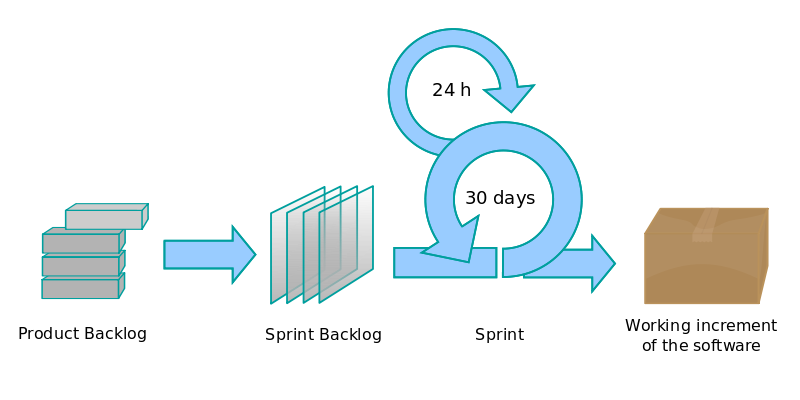
\includegraphics[scale=0.4]{pictures/Scrumprocess.png}
\end{figure}

\subsubsection{Scrum in the project}

This project will not follow the methodology to the letter. The reason for this is that the team do 
not have the opportunity to work together as much as would be preferred, with all members present. This affects
for example the Standup routine. Standups will not be held every day, the way one would do in the scrum,
but when the team sit together every member gives a status report of what they are working on. Even though standups are not held, it is still important to give the other team members a status update.

Allocation of roles has been limited to the Scrum master and the Scrum team where each person in the scrum team has an area of responsability. Sprint planning is run in advance of each sprint and a sprint delivery for the customer 
is held after each sprint. The objective of the sprint delivery is that the customer is able to see the results and progress of the project. During these deliveries the customer has the opportunity to present feedback and changes 
if they want to.

After each sprint a "sprint retrospective" is held to always strive for better working 
process. This allows the group members to give feedback to each other.

